\documentclass[tikz,border=12pt]{standalone}
\usepackage{amsmath}
\usetikzlibrary{arrows.meta,calc}

\begin{document}
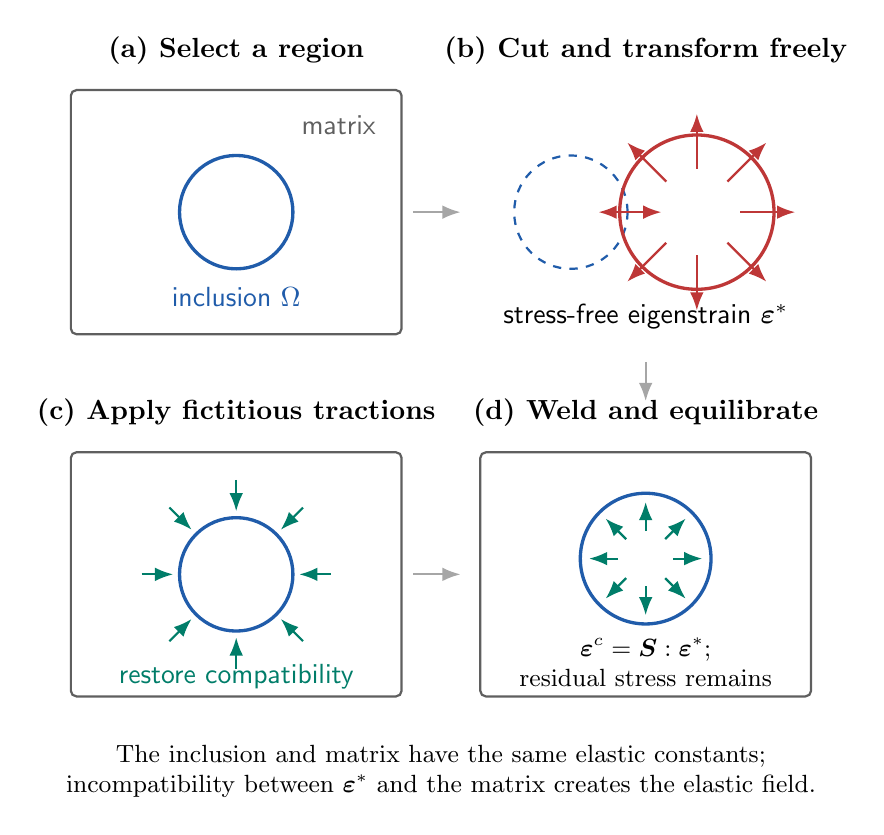
\begin{tikzpicture}[>=Latex,font=\sffamily,thick]
\definecolor{matrixcolor}{RGB}{95,95,95}
\definecolor{inclusion}{RGB}{32,92,170}
\definecolor{eigenstrain}{RGB}{190,55,55}
\definecolor{stress}{RGB}{0,125,105}

\newcommand{\matrixbox}[2]{
  \draw[matrixcolor,rounded corners=2pt] (#1,#2) rectangle ++(4.2,3.1);
}

% (a) Identify the region.
\begin{scope}[shift={(-4.7,2.0)}]
  \node[font=\bfseries] at (2.1,3.60) {(a) Select a region};
  \matrixbox{0}{0}
  \draw[inclusion,very thick] (2.1,1.55) circle (0.72);
  \node[inclusion] at (2.1,0.48) {inclusion $\Omega$};
  \node[matrixcolor] at (3.40,2.65) {matrix};
\end{scope}

% (b) Cut and allow stress-free transformation.
\begin{scope}[shift={(0.5,2.0)}]
  \node[font=\bfseries] at (2.1,3.60) {(b) Cut and transform freely};
  \draw[inclusion,dashed] (1.15,1.55) circle (0.72);
  \draw[eigenstrain,very thick] (2.75,1.55) circle (0.98);
  \draw[->,eigenstrain] (1.88,1.55)--(2.30,1.55);
  \foreach \ang in {0,45,...,315}{
    \draw[->,eigenstrain]
      ({2.75+0.55*cos(\ang)},{1.55+0.55*sin(\ang)})
      --({2.75+1.25*cos(\ang)},{1.55+1.25*sin(\ang)});
  }
  \node[align=center] at (2.1,0.22)
    {stress-free eigenstrain $\boldsymbol\varepsilon^*$};
\end{scope}

% (c) Restore the transformed region to the cavity size.
\begin{scope}[shift={(-4.7,-2.6)}]
  \node[font=\bfseries] at (2.1,3.60) {(c) Apply fictitious tractions};
  \matrixbox{0}{0}
  \draw[inclusion,very thick] (2.1,1.55) circle (0.72);
  \foreach \ang in {0,45,...,315}{
    \draw[->,stress]
      ({2.1+1.20*cos(\ang)},{1.55+1.20*sin(\ang)})
      --({2.1+0.80*cos(\ang)},{1.55+0.80*sin(\ang)});
  }
  \node[stress,align=center] at (2.1,0.25)
    {restore compatibility};
\end{scope}

% (d) Weld and remove the fictitious tractions.
\begin{scope}[shift={(0.5,-2.6)}]
  \node[font=\bfseries] at (2.1,3.60) {(d) Weld and equilibrate};
  \matrixbox{0}{0}
  \draw[inclusion,very thick] (2.1,1.75) circle (0.83);
  \foreach \ang in {0,45,...,315}{
    \draw[->,stress]
      ({2.1+0.35*cos(\ang)},{1.75+0.35*sin(\ang)})
      --({2.1+0.72*cos(\ang)},{1.75+0.72*sin(\ang)});
  }
  \node[align=center,font=\small] at (2.1,0.43)
    {$\boldsymbol\varepsilon^c=\boldsymbol S:\boldsymbol\varepsilon^*$;\\
     residual stress remains};
\end{scope}

\draw[->,gray!70] (-0.35,3.55)--(0.25,3.55);
\draw[->,gray!70] (2.60,1.65)--(2.60,1.15);
\draw[->,gray!70] (-0.35,-1.05)--(0.25,-1.05);

\node[font=\small,align=center] at (0,-3.55)
  {The inclusion and matrix have the same elastic constants;\\
   incompatibility between $\boldsymbol\varepsilon^*$ and the matrix creates the elastic field.};
\end{tikzpicture}
\end{document}
